
\section{Angles} 

\subsection*{Neighborhood angles}

Tim is walking around his neighborhood in St.\ Paul, obsessing about angles.  He sees angles, like, everywhere.  

Tim notices the stately oak, the energetic maple, and the perfectly formed linden tree all have branches sticking out at funny angles -- perhaps 45$^\circ$ for the linden, 60$^\circ$ for the maple, and up to 90$^\circ$ for the oak.

\begin{figure}[htbp]
    \centering   \includegraphics[width=0.5\linewidth]{Graphics/tree_branches.png}
    \caption{Branch angles. Source: Gemini}
    \label{fig_branch_angles}
\end{figure}

Tim compares the roof lines of the 1920s one-and-a-half story craftsman bungalows with their low-slung roofs at about 20$^\circ$ to the 1940s two-story tudors with their dramatic 40$^\circ$ pitched roofs.

\begin{figure} [htbp]
    \centering
    \includegraphics[width=0.6\linewidth]{Graphics/bungalow_tudor.png}
    \caption{Comparing roof angles on a bungalow (left) and tudor (right). Source: Gemini}
    \label{fig_roof_lines}
\end{figure}

He passes the local skate park and sees a few teens practicing their spins.  A quick 180$^\circ$ frontside (where you end up facing the opposite direction), a 360$^\circ$ aeriel (where you end up facing the same direction you started), and one kid even pulled off a 540$^\circ$ aeriel!

\begin{figure} [htbp]
    \centering
    \includegraphics[width=0.5\linewidth]{Graphics/skateboard.png}
    \caption{A 540 aerial on a skateboard.  Source: Gemini}
    \label{fig_540_aerial}
\end{figure}

\subsection*{Angles in triangles}

Tim learned in geometry class that angles can be measured between any two lines.  For example each pair of sides in a triangle has an angle between them.  A fun fact is that the three angles in a triangle add up to 180$^\circ$, the same number of degrees as a straight line.

For example, the triangular roof on the bungalow house has two angles of 20$^\circ$, which means the larger angle is $$180^\circ-20^\circ-20^\circ=140^\circ$$

\begin{center}
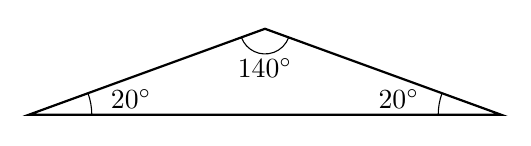
\begin{tikzpicture}[scale=1]
    % Coordinates
    \coordinate (A) at (0, 0);
    \coordinate (B) at (6, 0);
    % Height h = 3 * tan(20°) ≈ 1.092
    \coordinate (C) at (3, 1.092);

    % Draw Roof Triangle (unfilled / white background)
    \draw[thick] (A) -- (B) -- (C) -- cycle;

    % Bottom-left angle arc and lowered label (20°)
    \draw (0.8,0) arc (0:20:0.8);
    \node at (1.3, 0.2) {$20^\circ$};

    % Bottom-right angle arc and lowered label (20°)
    \draw (5.2,0) arc (180:160:0.8);
    \node at (4.7, 0.2) {$20^\circ$};

    % Top angle arc tighter to vertex (C), label lowered beneath the arc
    \draw (2.7, 0.983) arc (200:340:0.32);
    \node at (3, 0.6) {$140^\circ$};
\end{tikzpicture}
\end{center}

There's a name for a triangle where two angles are equal.  It's called an \textbf{isoceles} triangle.  The roof on the bungalow house (and the tudor house) form isoceles triangles.  A fun fact about isoceles triangles is that the sides across from the matching angles have the same length.  For example, the roof might have these dimensions.

\begin{center}
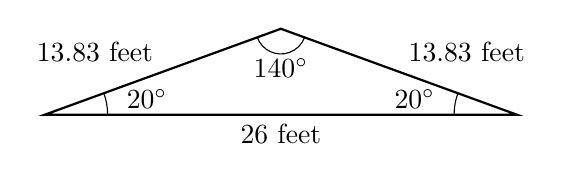
\begin{tikzpicture}[scale=1]
    % Coordinates
    \coordinate (A) at (0, 0);
    \coordinate (B) at (6, 0);
    % Height h = 3 * tan(20°) ≈ 1.092
    \coordinate (C) at (3, 1.092);

    % Draw Roof Triangle
    \draw[thick] (A) -- (B) -- (C) -- cycle;

    % Bottom-left angle arc and label (20°)
    \draw (0.8,0) arc (0:20:0.8);
    \node at (1.3, 0.2) {$20^\circ$};

    % Bottom-right angle arc and label (20°)
    \draw (5.2,0) arc (180:160:0.8);
    \node at (4.7, 0.2) {$20^\circ$};

    % Top angle arc and label (140°)
    \draw (2.7, 0.983) arc (200:340:0.32);
    \node at (3, 0.6) {$140^\circ$};

    % Side Labels
    \node[below] at (3, 0) {26 feet};
    \node[above left, sloped] at (1.5, 0.546) {13.83 feet};
    \node[above right, sloped] at (4.5, 0.546) {13.83 feet};
\end{tikzpicture}
\end{center}

\subsection*{A Special Triangle}
The 60$^\circ$ of the maple tree branch  sits within a right triangle.  The missing angle is $$180^\circ-90^\circ-60^\circ = 30^\circ.$$
Notice if we measure $a=1$ foot up the tree and $b$ feet out from the tree, it's not immediately clear what $b$ equals. We can label the length of the corresponding branch $c$ feet.

\begin{center}
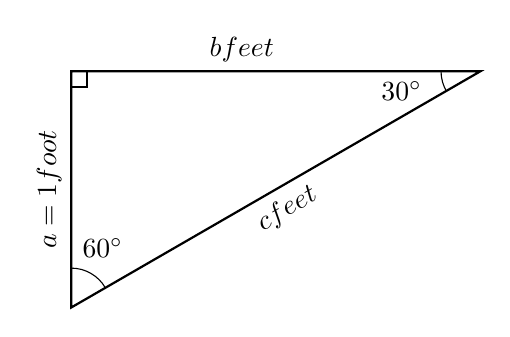
\begin{tikzpicture}[scale=1]
    % Coordinates
    \coordinate (A) at (0, 3);          % Right-angle corner (top-left)
    \coordinate (B) at (0, 0);          % Bottom corner
    \coordinate (C) at (1.732*3, 3);    % Top-right corner (b = sqrt(3) ≈ 1.732 relative to a = 1)

    % Draw Triangle (a=1 vertical leg, b=sqrt(3) horizontal top leg, c=2 hypotenuse)
    \draw[thick] (A) -- (C) -- (B) node[midway, sloped, below] {$c \text{ feet}$} -- cycle;

    % Right angle symbol
    \draw (0, 2.8) -- (0.2, 2.8) -- (0.2, 3);

    % Bottom-left 60° angle arc and label
    \draw (0, 0.5) arc (90:30:0.5);
    \node at (0.4, 0.75) {$60^\circ$};

    % Top-right 30° angle arc and label
    \draw (1.732*3 - 0.5, 3) arc (180:210:0.5);
    \node at (1.732*3 - 1, 2.75) {$30^\circ$};

    % Side Labels
    \node[left, rotate=90, anchor=south] at (0, 1.5) {$a = 1\text{ foot}$};
    \node[above] at (1.732*1.25, 3) {$b\text{ feet}$};
\end{tikzpicture}
\end{center}

Let's figure out what $b$ and $c$ are.  Look what happens if we put an upside-down copy of the triangle on top of our triangle. 

\begin{center}
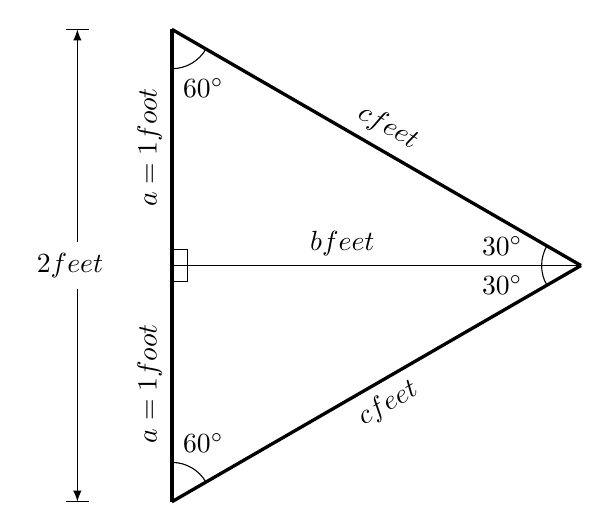
\begin{tikzpicture}[scale=1]
    % Coordinates for Bottom Triangle
    \coordinate (A) at (0, 3);          % Shared Right-angle corner
    \coordinate (B) at (0, 0);          % Bottom-left corner
    \coordinate (C) at (1.732*3, 3);    % Far-right corner

    % Coordinates for Top Triangle
    \coordinate (B2) at (0, 6);         % Top-left corner

    % --- BOTTOM TRIANGLE ---
    % Base (b) normal thickness, sides (a and c) made very thick
    \draw (A) -- (C);
    \draw[very thick] (C) -- (B) node[midway, sloped, below] {$c\text{ feet}$};
    \draw[very thick] (A) -- (B);

    % Bottom triangle right angle symbol
    \draw (0, 2.8) -- (0.2, 2.8) -- (0.2, 3);

    % Bottom-left 60° angle arc and label
    \draw (0, 0.5) arc (90:30:0.5);
    \node at (0.4, 0.75) {$60^\circ$};

    % Bottom top-right 30° angle arc and label
    \draw (1.732*3 - 0.5, 3) arc (180:210:0.5);
    \node at (1.732*3 - 1, 2.75) {$30^\circ$};

    % Bottom side label (rotated sideways)
    \node[left, rotate=90, anchor=south] at (0, 1.5) {$a = 1\text{ foot}$};

    % --- TOP TRIANGLE ---
    \draw[very thick] (C) -- (B2) node[midway, sloped, above] {$c \text{ feet}$};
    \draw[very thick] (A) -- (B2);

    % Top triangle right angle symbol
    \draw (0, 3.2) -- (0.2, 3.2) -- (0.2, 3);

    % Top-left 60° angle arc and label
    \draw (0, 5.5) arc (270:330:0.5);
    \node at (0.4, 5.25) {$60^\circ$};

    % Top top-right 30° angle arc and label
    \draw (1.732*3 - 0.5, 3) arc (180:150:0.5);
    \node at (1.732*3 - 1, 3.25) {$30^\circ$};

    % Top side label (rotated sideways)
    \node[left, rotate=90, anchor=south] at (0, 4.5) {$a = 1\text{ foot}$};

    % --- SHARED MIDDLE SIDE LABEL (b) ---
    \node[above] at (1.732*1.25, 3) {$b\text{ feet}$};

    % --- FULL LENGTH DIMENSION BAR (2 feet) ---
    % Dimension line shifted left to x = -1.2
    \draw[<-, >=latex] (-1.2, 0) -- (-1.2, 2.7);
    \draw[->, >=latex] (-1.2, 3.3) -- (-1.2, 6);
    % End caps (ticks) at top and bottom
    \draw (-1.35, 0) -- (-1.05, 0);
    \draw (-1.35, 6) -- (-1.05, 6);
    % Text label centered along the dimension bar
    \node[left] at (-.75, 3) {$2\text{ feet}$};
\end{tikzpicture}
\end{center}

Notice that the sides labeled $b$ line up and the sides labeled $a$ fall exactly in a straight line because $$90^\circ + 90^\circ = 180^\circ$$ That entire side of the big outer triangle is length $1+1=2$ feet.

The angles of the outer triangle are $60^\circ$, $60^\circ$, and $30^\circ + 30^\circ=60^\circ$, which means all three angles are equal.  By symmetry, the lengths of the sides must all be equal too.   Since the left-hand side has length 2 feet, we get $c=2$ feet also.

By the way, when all three angles and all three sides of a triangle are equal, it is an \textbf{equilateral triangle}. So an isoceles triangles has two angles and two sides equal, but an equilateral triangle has three angles and three sides equal.

Let's go back to our original triangle and use the Pythagorean Theorem to find the length $b$.  We know
$$a^2 + b^2 = c^2.$$
Evaluating at $a=1$ and $c=2$ we get
and so $$1^2 + b^2 = 2^2$$  That is,
$$1 + b^2 = 4$$
so subtracting 1 from each side we get
$b^2 = 3$.  Therefore $b = \sqrt{3} \approx 1.732 \text{ feet}$.

\begin{center}
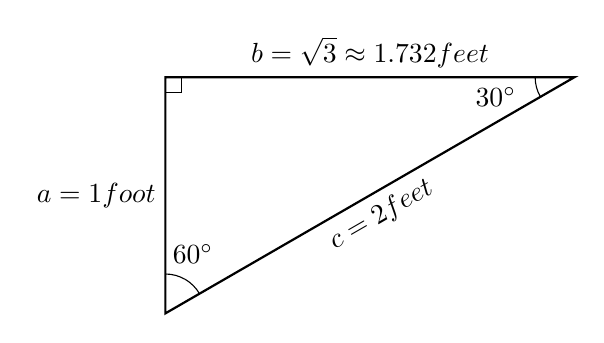
\begin{tikzpicture}[scale=1]
    % Coordinates
    \coordinate (A) at (0, 3);          % Right-angle corner (top-left)
    \coordinate (B) at (0, 0);          % Bottom corner
    \coordinate (C) at (1.732*3, 3);    % Top-right corner (b = sqrt(3) ≈ 1.732 relative to a = 1)

    % Draw Triangle (a=1 vertical leg, b=sqrt(3) horizontal top leg, c=2 hypotenuse)
    \draw[thick] (A) -- (C) -- (B) node[midway, sloped, below] {$c = 2\text{ feet}$} -- cycle;

    % Right angle symbol
    \draw (0, 2.8) -- (0.2, 2.8) -- (0.2, 3);

    % Bottom-left 60° angle arc and label
    \draw (0, 0.5) arc (90:30:0.5);
    \node at (0.35, 0.75) {$60^\circ$};

    % Top-right 30° angle arc and label
    \draw (1.732*3 - 0.5, 3) arc (180:210:0.5);
    \node at (1.732*3 - 1, 2.75) {$30^\circ$};

    % Side Labels
    \node[left] at (0, 1.5) {$a = 1\text{ foot}$};
    \node[above] at (1.732*1.5, 3) {$b = \sqrt{3} \approx 1.732\text{ feet}$};
\end{tikzpicture}
\end{center}

This is a \textbf{special triangle} because there were nice clean numbers for the lengths.  In a precalculus or calculus class, you might see this triangle drawn in various positions. 

\begin{center}
%% Triangle in branch position
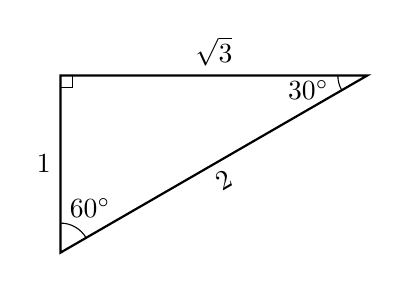
\begin{tikzpicture}[scale=.75]
    % Coordinates
    \coordinate (A) at (0, 3);          % Right-angle corner (top-left)
    \coordinate (B) at (0, 0);          % Bottom corner
    \coordinate (C) at (1.732*3, 3);    % Top-right corner (b = sqrt(3) ≈ 1.732 relative to a = 1)

    % Draw Triangle (a=1 vertical leg, b=sqrt(3) horizontal top leg, c=2 hypotenuse)
    \draw[thick] (A) -- (C) -- (B) node[midway, sloped, below] {2} -- cycle;

    % Right angle symbol
    \draw (0, 2.8) -- (0.2, 2.8) -- (0.2, 3);

    % Bottom-left 60° angle arc and label
    \draw (0, 0.5) arc (90:30:0.5);
    \node at (0.5, 0.75) {$60^\circ$};

    % Top-right 30° angle arc and label
    \draw (1.732*3 - 0.5, 3) arc (180:210:0.5);
    \node at (1.732*3 - 1, 2.75) {$30^\circ$};

    % Side Labels
    \node[left] at (0, 1.5) {1};
    \node[above] at (1.732*1.5, 3) {$ \sqrt{3}$};
\end{tikzpicture}
\hfill %%%%%%%%
%% Triangle in standard 60 degree position
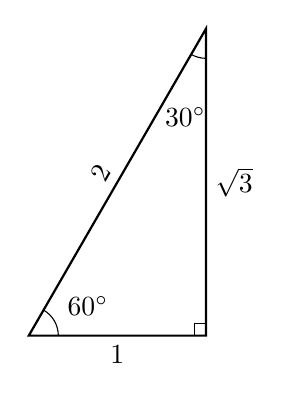
\begin{tikzpicture}[scale=.75]
    % Coordinates: 
    % Side 1 (horizontal): length = 3
    % Side \sqrt{3} (vertical to the right): length = 1.732 * 3 ≈ 5.196
    \coordinate (A) at (3, 0);          % Right-angle corner (bottom-right)
    \coordinate (B) at (0, 0);          % Bottom-left corner
    \coordinate (C) at (3, 1.732*3);    % Top-right corner

    % Draw Triangle
    \draw[thick] (A) -- (B) -- (C) node[midway, sloped, above] {2} -- cycle;

    % Right angle symbol (at bottom-right)
    \draw (2.8, 0) -- (2.8, 0.2) -- (3, 0.2);

    % Bottom-left 60° angle arc and label
    \draw (0.5, 0) arc (0:60:0.5);
    \node at (1, 0.5) {$60^\circ$};

    % Top-right 30° angle arc and label
    \draw (3, 1.732*3 - 0.5) arc (270:240:0.5);
    \node at (2.65, 1.732*3 - 1.5) {$30^\circ$};

    % Side Labels
    \node[below] at (1.5, 0) {1};
    \node[right] at (3, 1.732*1.5) {$\sqrt{3}$};
\end{tikzpicture}
\hfill %%%%%%%%
%% Triangle in standard 30 degree position
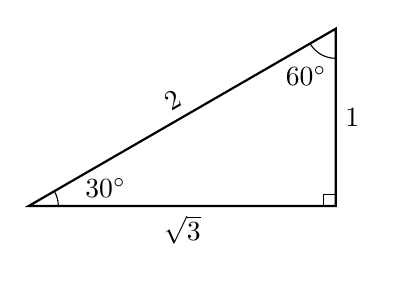
\begin{tikzpicture}[scale=.75]
    % Coordinates:
    % Side \sqrt{3} (horizontal bottom): length = 1.732 * 3 ≈ 5.196
    % Side 1 (vertical to the right): length = 3
    \coordinate (A) at (1.732*3, 0);    % Right-angle corner (bottom-right)
    \coordinate (B) at (0, 0);          % Bottom-left corner
    \coordinate (C) at (1.732*3, 3);    % Top-right corner

    % Draw Triangle
    \draw[thick] (A) -- (B) -- (C) node[midway, sloped, above] {2} -- cycle;

    % Right angle symbol (at bottom-right)
    \draw (1.732*3 - 0.2, 0) -- (1.732*3 - 0.2, 0.2) -- (1.732*3, 0.2);

    % Bottom-left 30° angle arc and label
    \draw (0.5, 0) arc (0:30:0.5);
    \node at (1.3, 0.3) {$30^\circ$};

    % Top-right 60° angle arc and label
    \draw (1.732*3, 3 - 0.5) arc (270:210:0.5);
    \node at (1.732*3 - 0.5, 2.2) {$60^\circ$};

    % Side Labels
    \node[below] at (1.732*1.5, 0) {$\sqrt{3}$};
    \node[right] at (1.732*3, 1.5) {1};
\end{tikzpicture}
\end{center}

In this \textbf{30-60-90 triangle}, the hypotenuse is always length 2, the shortest side (of length 1) is across from (or ``opposite'') to the smaller $30^\circ$ angle, and the longer side opposite to the larger $60^\circ$ angle is length $\sqrt{3}$.

You will see another special triangle, the \textbf{isoceles right triangle} (or \textbf{45-45-90 triangle}, in the exercises.

\subsection*{Angles in Standard Position}

Not all angles fit in a right triangle or even any shape triangle.  Like that 540$^\circ$ rotation of the skateboarder.  A general way to measure angles is to start the measure on the positive horizontal axis, let's label it the $x$-axis and rotate counterclockwise around.  In case you're not familiar with the hands on an analog clock, that means we head towards the positive vertical axis, which we'll label the $y$-axis.  For example, the picture shows measuring angles of $30^\circ$, $45^\circ$, $60^\circ$,  $90^\circ$, and $180^\circ$.



\begin{center}
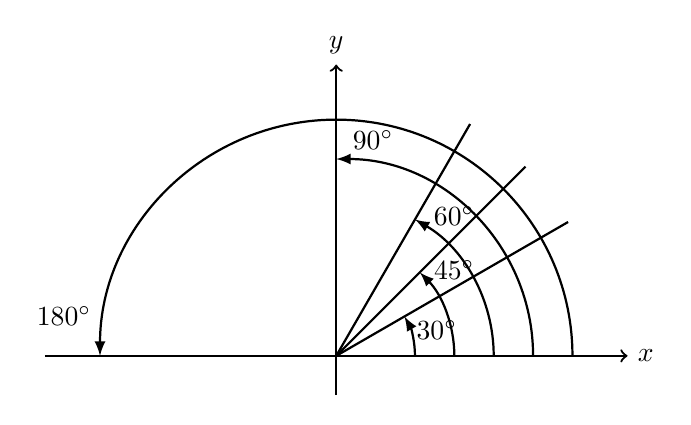
\begin{tikzpicture}[scale=1]
    % Draw Axes (without tick marks)
    \draw[->, thick] (-3.7, 0) -- (3.7, 0) node[right] {$x$};
    \draw[->, thick] (0, -0.5) -- (0, 3.7) node[above] {$y$};

    % --- 30° Angle ---
    \draw[thick] (0, 0) -- (30:3.4);
    \draw[->, >=latex, line width=0.8pt] (1.0, 0) arc (0:30:1.0);
    \node[above right] at (5:0.9) {$30^\circ$};

    % --- 45° Angle ---
    \draw[thick] (0, 0) -- (45:3.4);
    \draw[->, >=latex, line width=0.8pt] (1.5, 0) arc (0:45:1.5);
    \node[above right] at (37:1.4) {$45^\circ$};

    % --- 60° Angle ---
    \draw[thick] (0, 0) -- (60:3.4);
    \draw[->, >=latex, line width=0.8pt] (2.0, 0) arc (0:60:2);
    \node[above right] at (54:1.9) {$60^\circ$};

    % --- 90° Angle ---
    % Terminal side lies on positive y-axis
    \draw[->, >=latex, line width=0.8pt] (2.5, 0) arc (0:90:2.5);
    \node[above right] at (88:2.5) {$90^\circ$};

    % --- 180° Angle ---
    % Terminal side lies on negative x-axis
    \draw[->, >=latex, line width=0.8pt] (3.0, 0) arc (0:180:3.0);
    \node[above left] at (175:3.0) {$180^\circ$};
\end{tikzpicture}
\end{center}

Note that the straight angle, 180$^\circ$, is halfway around the circle.  A full rotation is 360$^\circ$.  That 540?  It's one and half times around because $$360^\circ + 180^\circ = 540^\circ$$
In our picture we also include three quarters of the way around which is $3 \times 90^\circ = 270^\circ$
Note that 0$^\circ$ is just where we start.

\begin{center}
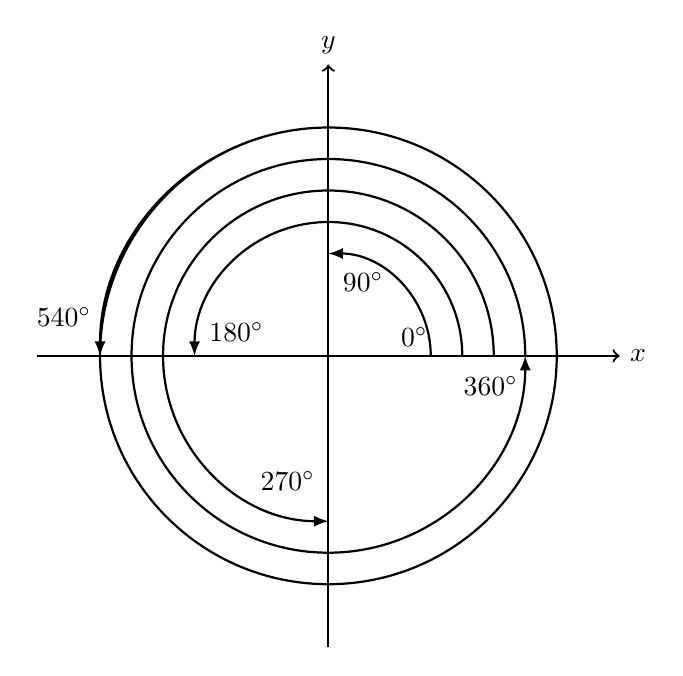
\begin{tikzpicture}[scale=1]
    % Draw Axes (without tick marks)
    \draw[->, thick] (-3.7, 0) -- (3.7, 0) node[right] {$x$};
    \draw[->, thick] (0, -3.7) -- (0, 3.7) node[above] {$y$};

    % --- 0° Angle ---
    % Terminal side lies on positive x-axis (no arc)
    \node[above right] at (0.8, 0) {$0^\circ$};

    % --- 90° Angle ---
    % Terminal side lies on positive y-axis
    \draw[->, >=latex, line width=0.8pt] (1.3, 0) arc (0:90:1.3);
    \node[above right] at (85:0.7) {$90^\circ$};

    % --- 180° Angle ---
    % Terminal side lies on negative x-axis
    \draw[->, >=latex, line width=0.8pt] (1.7, 0) arc (0:180:1.7);
    \node[above left] at (175:.7) {$180^\circ$};

    % --- 270° Angle ---
    % Terminal side lies on negative y-axis
    \draw[->, >=latex, line width=0.8pt] (2.1, 0) arc (0:270:2.1);
    \node[below left] at (268:1.35) {$270^\circ$};

    % --- 360° Angle ---
    % Full rotation back to positive x-axis
    \draw[->, >=latex, line width=0.8pt] (2.5, 0) arc (0:360:2.5);
    \node[below right] at (355:1.6) {$360^\circ$};

    % --- 540° Angle ---
    % 1.5 full rotations (ends on negative x-axis)
    \draw[->, >=latex, line width=0.8pt] (2.9, 0) arc (0:540:2.9);
    \node[above left] at (175:2.9) {$540^\circ$};
\end{tikzpicture}
\end{center}

We can even talk about negative angles if we imagine they rotate clockwise (the other direction) instead.

\begin{center}
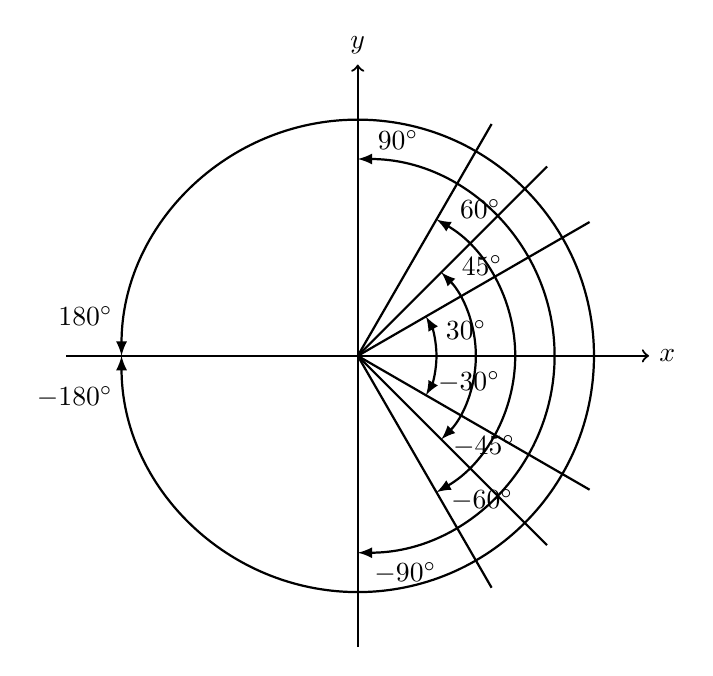
\begin{tikzpicture}[scale=1]
    % Draw Axes (without tick marks)
    \draw[->, thick] (-3.7, 0) -- (3.7, 0) node[right] {$x$};
    \draw[->, thick] (0, -3.7) -- (0, 3.7) node[above] {$y$};

    % ================= POSITIVE ANGLES =================
    % --- 30° Angle ---
    \draw[thick] (0, 0) -- (30:3.4);
    \draw[->, >=latex, line width=0.8pt] (1.0, 0) arc (0:30:1.0);
    \node[above right] at (5:1.0) {$30^\circ$};

    % --- 45° Angle ---
    \draw[thick] (0, 0) -- (45:3.4);
    \draw[->, >=latex, line width=0.8pt] (1.5, 0) arc (0:45:1.5);
    \node[above right] at (37:1.5) {$45^\circ$};

    % --- 60° Angle ---
    \draw[thick] (0, 0) -- (60:3.4);
    \draw[->, >=latex, line width=0.8pt] (2.0, 0) arc (0:60:2.0);
    \node[above right] at (54:2.0) {$60^\circ$};

    % --- 90° Angle ---
    \draw[->, >=latex, line width=0.8pt] (2.5, 0) arc (0:90:2.5);
    \node[above right] at (87:2.5) {$90^\circ$};

    % --- 180° Angle ---
    \draw[->, >=latex, line width=0.8pt] (3.0, 0) arc (0:180:3.0);
    \node[above left] at (175:3.0) {$180^\circ$};

    % ================= NEGATIVE ANGLES =================
    % --- -30° Angle ---
    \draw[thick] (0, 0) -- (-30:3.4);
    \draw[->, >=latex, line width=0.8pt] (1.0, 0) arc (0:-30:1.0);
    \node[below right] at (-5:0.9) {$-30^\circ$};

    % --- -45° Angle ---
    \draw[thick] (0, 0) -- (-45:3.4);
    \draw[->, >=latex, line width=0.8pt] (1.5, 0) arc (0:-45:1.5);
    \node[below right] at (-39:1.4) {$-45^\circ$};

    % --- -60° Angle ---
    \draw[thick] (0, 0) -- (-60:3.4);
    \draw[->, >=latex, line width=0.8pt] (2.0, 0) arc (0:-60:2.0);
    \node[below right] at (-56:1.9) {$-60^\circ$};

    % --- -90° Angle ---
    % Terminal side lies on negative y-axis
    \draw[->, >=latex, line width=0.8pt] (2.5, 0) arc (0:-90:2.5);
    \node[below right] at (-88:2.5) {$-90^\circ$};

    % --- -180° Angle ---
    % Terminal side lies on negative x-axis
    \draw[->, >=latex, line width=0.8pt] (3.0, 0) arc (0:-180:3.0);
    \node[below left] at (-175:3.0) {$-180^\circ$};
\end{tikzpicture}
\end{center}

When we draw an angle starting on the positive $x$-axis and rotate counterclockwise for a positive angle and clockwise for a negative angle, we say the angle is drawn \textbf{in standard position}.

\subsection*{Naming angles with Greek letters}

Textbooks often name angles using Greek letters. Two commonly used Greek letters are
$$\alpha \text{ (alpha, pronounced ``al-fah")}$$
$$\beta \text{ (beta, pronounced ``bay-tah")}$$ 
They are like the letters $a$ and $b$, the first two letters of the alphabet.  In fact, the word ``alphabet'' comes from the Greek language.  So now you know. 

Some other common Greek letter names for angles are
$$\gamma \text{ (gamma, pronounced ``gam-uh")}$$
$$\theta \text{ (theta, pronounced ``thay-tah")}$$
$$\phi \text{ (phi, pronounced ``fee")}$$

 \input{GoDoWS}

\noindent \textbf{Do you know \ldots}

\begin{itemize}
\item Do you know what the sum of the angles inside a triangle is?
\item How to draw angles in ``standard position'' including negative angles?
\item How many degrees are in a straight line angle?
\item How many degrees are in a full circle?
\item How to use the Pythagorean theorem to the length of a side of a right triangle, if you know the lengths of the other two sides?
\item How to draw and label the standard 30-60-90 triangle?
\item How to draw and label the 45-45-90 (isoceles right triangle)?
 \input{NotSure} 
\end{itemize}

\subsection*{Exercises}

\begin{enumerate} 
\item %workbook
Find the missing angle in each triangle.

\begin{enumerate}
    \item What is the center angle $\alpha$ on the roof of a tudor house?

    \begin{center}
       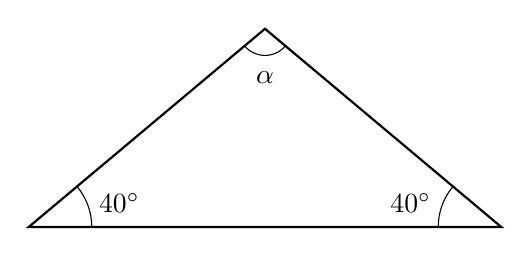
\begin{tikzpicture}[scale=1]
    % Coordinates
    \coordinate (A) at (0, 0);
    \coordinate (B) at (6, 0);
    % Height h = 3 * tan(40°) ≈ 2.517
    \coordinate (C) at (3, 2.517);

    % Draw Roof Triangle
    \draw[thick] (A) -- (B) -- (C) -- cycle;

    % Bottom-left angle arc and label (40°)
    \draw (0.8,0) arc (0:40:0.8);
    \node at (1.15, 0.3) {$40^\circ$};

    % Bottom-right angle arc and label (40°)
    \draw (5.2,0) arc (180:140:0.8);
    \node at (4.85, 0.3) {$40^\circ$};

    % Top angle arc (unlabeled)
    \draw (2.74, 2.3) arc (220:320:0.34);
    \node at (3,1.9) {$\alpha$};
\end{tikzpicture}
    \end{center}
    
    \item What is the center angle $\beta$ on the roof of a Gothic Revival house?
    \begin{center}
        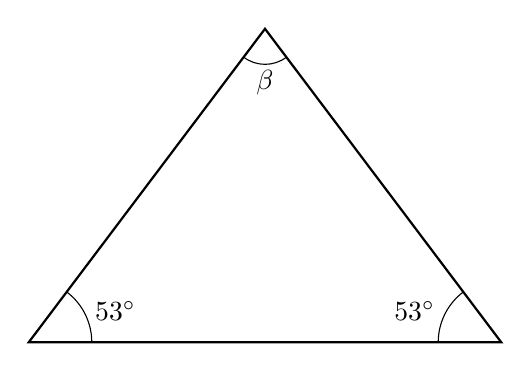
\begin{tikzpicture}[scale=1]
    % Coordinates
    \coordinate (A) at (0, 0);
    \coordinate (B) at (6, 0);
    % Height h = 3 * tan(53°) ≈ 3.981
    \coordinate (C) at (3, 3.981);

    % Draw Roof Triangle
    \draw[thick] (A) -- (B) -- (C) -- cycle;

    % Bottom-left angle arc and label (53°)
    \draw (0.8,0) arc (0:53:0.8);
    \node at (1.1, 0.4) {$53^\circ$};

    % Bottom-right angle arc and label (53°)
    \draw (5.2,0) arc (180:127:0.8);
    \node at (4.9, 0.4) {$53^\circ$};

    % Top angle arc (unlabeled)
    \draw (2.73, 3.62) arc (233:307:0.45);
    \node at (3,3.3) {$\beta$};
\end{tikzpicture}
    \end{center}

    \item Marta is climbing is hanging a banner for Coach Pelto. The 16-foot ladder makes an angle of approximately 75.5$^\circ$ with the floor.  What angle $\theta$ does the ladder make with the wall? \hfill \emph{Story appears in 6.2}

     \begin{center}
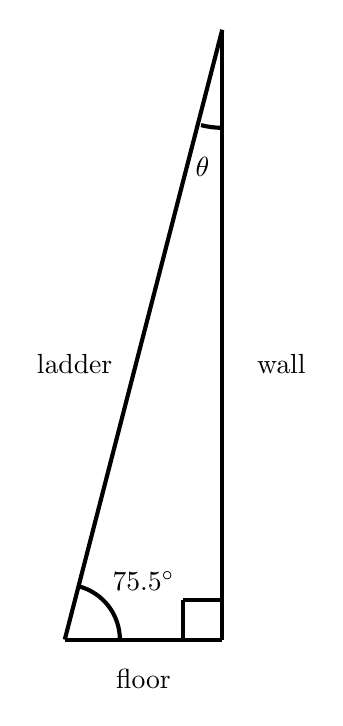
\begin{tikzpicture}[line width=1.5pt, scale = .5]
    % The triangle
    \draw (0,0) -- (4,0);
    \draw (4,0) -- (4,15.491);
    \draw (0,0) -- (4,15.491);

    % Labels
    \node at (2, -1) {floor};
    \node at (0.25, 7) {ladder};
    \node at (5.5, 7) {wall};

    % Box indicating perpendicular
    \draw (3,1) -- (4,1);
    \draw (3,0) -- (3,1);

    % Bottom-left angle arc and label (14.5°)
    \draw (1.4, 0) arc (0:75.5:1.4);
    \node at (2, 1.5) {$75.5^\circ$};

    % Top angle arc and label (B)
    \draw (4, 13) arc (270:255.5:2.15);
    \node at (3.5, 12) {$\theta$};
\end{tikzpicture}
 \end{center}

 \item An ADA accessible ramp is 48 feet long and rises 4 feet from the sidewalk to the entrance to the women's health clinic.  If the ramp makes an angle of approximately $4.78^\circ$ with the ground, at what angle $\phi$ does the ramp meet the entrance?
 \hfill \emph{Story also appears in 6.2}

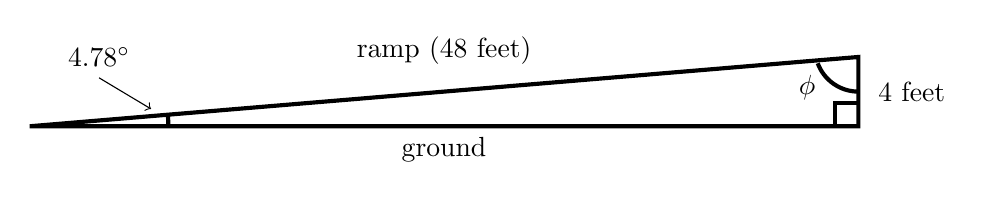
\begin{tikzpicture}[line width=1.5pt, scale=0.22]
    % Coordinates: width ≈ 47.83 ft, height = 4 ft
    \coordinate (A) at (0, 0);
    \coordinate (B) at (47.833, 0);
    \coordinate (C_coord) at (47.833, 4);

    % Draw Triangle
    \draw (A) -- (B) -- (C_coord) -- cycle;

    % Right angle indicator square at (B), scaled down to 2/3 size
    \pgfmathsetmacro{\sqSize}{2 * 2/3}
    \pgfmathsetmacro{\cornerX}{47.833 - \sqSize}
    \draw (\cornerX, 0) -- (\cornerX, \sqSize) -- (47.833, \sqSize);

    % Side Labels
    \node[below] at (23.916, 0) {ground};
    \node[right] at (48.333, 2) {4 feet};
    \node[above left, sloped, anchor=south, yshift=2mm] at (23.916, 2) {ramp (48 feet)};

    % Angle at bottom-left arc
    \draw (8, 0) arc (0:4.78:8);

    % (1) 4.78° moved closer (x=-2, y=2.2) and arrow re-aimed to arc
    \node (angleLabel) at (4, 4) {$4.78^\circ$};
    \draw[->, thin] (angleLabel.south) -- (7, 1);

    % Angle arc at top vertex C
    \draw (47.833, 2) arc (270:200.22:2.5);
    % (2) Label C moved higher (y=2.6) while keeping it under the arc
    \node[below left] at (46.0, 3.6) {$\phi$};
\end{tikzpicture}
\end{enumerate}

\item % workbook DRAWING ANGLES in std position
Valeria is just learning to skateboard. She is trying to do a full 360$^\circ$ but she's not quite there yet.  Draw each angle Valeria was able to land in standard position.
\begin{enumerate}
    \item $80^\circ$
    \item $150^\circ$
    \item $225^\circ$  Hint: $225 = 180 + 45$.
    \item $300^\circ$  So close!
\end{enumerate}
\item % workbook
The 45$^\circ$ of the linden tree branch also sits within a right triangle.  If we measure $a=1$ foot vertically up the tree and then $b$ feet out horizontally to meet the branch, of length $c$ feet, then we get this triangle.

\begin{center}
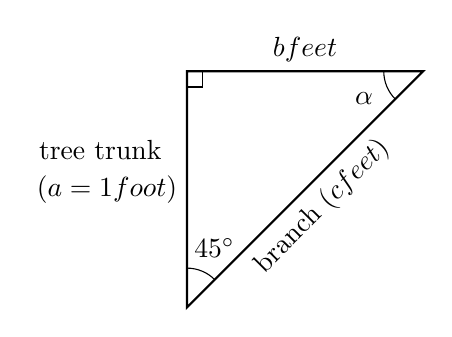
\begin{tikzpicture}[scale=1]
    % Coordinates
    \coordinate (A) at (0, 3); % Right-angle corner (top-left)
    \coordinate (B) at (0, 0); % Bottom corner
    \coordinate (C) at (3, 3); % Top-right corner

    % Draw Triangle with hypotenuse label attached
    \draw[thick] (A) -- (C) -- (B) node[midway, sloped, below] {branch ($c \text{ feet}$)} -- cycle;

    % Right angle symbol
    \draw (0, 2.8) -- (0.2, 2.8) -- (0.2, 3);

    % Bottom 45° angle arc and label
    \draw (0, 0.5) arc (90:45:0.5);
    \node at (0.35, 0.75) {$45^\circ$};

    % Top-right 45° angle arc and label
    \draw (2.5, 3) arc (180:225:0.5);
    \node at (2.25, 2.65) {$\alpha$};

    % Side Labels
    \node[left] at (0, 1.5) {($a = 1\text{ foot}$)};
    \node[left] at (-.2, 2) {tree trunk};
    \node[above] at (1.5, 3) {$b \text{ feet}$};
\end{tikzpicture}
\end{center}

\begin{enumerate}
    \item Find the missing angle $\alpha$.
    \item Use symmetry to explain why $b=1$ foot.   
    \item Use the Pythagorean Theorem to find $c$, the length of the branch.  Give an exact answer (using square roots) and an approximation to three decimal places.
    \item Redraw the triangle in a new position where one leg is horizontal at the bottom and the other leg is vertical on the right.  Label each side with their length and use the exact square root value for the hypotenuse. Label the angles including drawing the small square at the right angle. This triangle is the \textbf{isoceles right triangle}.
\end{enumerate}

\item % workbook
Suba is tossing and turning.  Can't sleep!  She looks at the clock and it says 2:50 AM (and 20 seconds). Argh.  Suba wonders, what angle each of the clock hands has traveled since midnight when she went to bed?  

\begin{center}
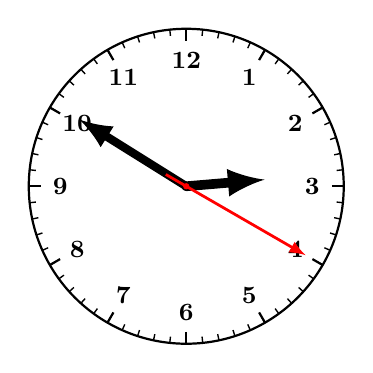
\begin{tikzpicture}[scale=1]
    % Clock face outline
    \draw[thick] (0,0) circle (2);
    \fill (0,0) circle (0.06); % Center pin

    % Hour ticks and numbers
    \foreach \angle/\label in {
        90/12, 60/1, 30/2, 0/3, 330/4, 300/5, 
        270/6, 240/7, 210/8, 180/9, 150/10, 120/11
    } {
        \draw[thick] (\angle:1.85) -- (\angle:2);
        \node at (\angle:1.6) {\small\textbf{\label}};
    }

    % Minute ticks (smaller)
    \foreach \m in {0,6,...,354} {
        \draw[line width=0.5pt] (\m:1.92) -- (\m:2);
    }

    % --- HAND CALCULATIONS ---
    % 2:50 and 20 seconds:
    % Hour hand angle = 90° - (2 + 50/60 + 20/3600) * 30° ≈ 4.83°
    % Minute hand angle = 90° - (50 + 20/60) * 6° = -212° = 148°
    % Second hand angle = 90° - (20 * 6°) = -30° = 330°

    % Hour hand (Short & Very Thick with Arrowhead)
    \draw[->, >=latex, line width=3.5pt, line cap=round] (0,0) -- (4.83:1.0);

    % Minute hand (Long & Very Thick with Arrowhead)
    \draw[->, >=latex, line width=3pt, line cap=round] (0,0) -- (148:1.6);

    % Second hand (Thin & Red with Arrowhead)
    \draw[->, >=latex, line width=1pt, red, line cap=round] (0,0) -- (330:1.75);
    \draw[line width=1pt, red] (0,0) -- (150:0.3); % Small tail
    \fill[red] (0,0) circle (0.04); % Red center cap
\end{tikzpicture}
\end{center}

All hands start pointing to 12 at midnight.  Notice the numbers 1, 2, \ldots 12 are placed equally around the circle.
\begin{enumerate}
    \item What is the angle between any two numbers on the clock (like 12 and 1 or 2 and 2)?
    \item The hour hand is the short thick arrow that points in between 2 and 3 (because it's almost 3 AM).  Approximately what angle has the hour hand traveled?  Hint: It moves from 12 to where it is.
    \item The minute hand is the long thick arrow that points at 10 (because it's $10 \times 5 = 50$ minutes past the hour.  Approximately what angle has the minute hand traveled?  Hint: It has made a full circle each hour (12-1, 1-2), plus the angle traveled from 12 to where it is now.
    \item The second hand is the long thin arrow that points to 4 (because it's $4 \times 5 = 20$ seconds past the hour). Hint: It has made a full circle each of the 170 minutes, plus the angle traveled from 12 to where it is now.
\end{enumerate}

\item % homework % A triangle with missing angle
In a sailboat race, the boats must navigate around three buoys (A, B, and C) forming a triangular course on the bay.  At buoy A, the angle between the line to B and the line to C measures 42$^\circ$.  At buoy B, the angle between the line to A and the line to C measures $68^\circ$.  At buoy C, what is the angle between the line to A and the line to B?

% \item % homework
% Drawing angles in standard position that include negative angles.
\item In a fantasy video game, a wizard aims spells relative to the horizontal ground.  That means, the positive $x$-axis is $0^\circ$.
\begin{enumerate}
    \item To cast a fire spell at a dragon flying in the sky, the wizard aims up at an angle of $115^\circ$. Draw this angle in standard position.
    \item To cast an ice spell at a creature on the ground below, the wizard aims down at an angle of $-60^\circ$. Draw this angle in standard position.
    \item If the wizard aims straight up into the air to launch a signal flare, what angle in standard position represents this direction?
\end{enumerate}

% \item % homework
% Something rotating a lot
\item At an amusement park, a giant swing ride starts facing directly east (along the positive $x$-axis, $0^\circ$).
\begin{enumerate}
    \item During a thrill ride, the swing spins counterclockwise through 2 full rotations plus another $45^\circ$. What is the total angle of rotation in degrees? Draw this angle in standard position.
    \item The swing returns to facing directly east.  Then, the swing spins counterclockwise through a total angle of $810^\circ$. How many full rotations does the swing complete, and where does it end up pointing?
    \item The swing returns to facing directly east.  Then, the swing spins counterclockwise through a total angle of $-450^\circ$ (which means it goes backwards $450^\circ$). Draw this angle in standard position.
\end{enumerate}

\end{enumerate}

\bigskip

\noindent \textbf{When you're done \ldots}

\begin{itemize}
\item Don't forget to check your answers with those in the back of the textbook. 
\item Not sure if your answers are close enough? Compare with a classmate or ask the instructor.  
\item Getting the wrong answers or stuck on a problem?  Re-read the section and try the problem again.  If you're still stuck, work with a classmate or go to your instructor's office hours.
\item It's normal to find some parts of some problems difficult, but if all the problems are giving you grief, be sure to talk with your instructor or advisor about it.  They might be able to suggest strategies or support services that can help you succeed.
\item Make a list of key ideas or processes to remember from the section.  The ``Do you know?'' questions can be a good starting point.
\end{itemize}



